\documentclass[11pt]{article}
\usepackage[margin=1in]{geometry}
\usepackage{enumitem}
\usepackage{hyperref}
\usepackage{graphicx}
\usepackage{array}
\usepackage{multicol}
\usepackage{longtable}
\usepackage{titlesec}
\usepackage{listings}
\usepackage{xcolor}
\usepackage[a4paper, margin=1in]{geometry}
\usepackage{float}      % For [H] placement
\usepackage{caption}
\usepackage{subcaption}
\usepackage{amsmath}
\usepackage{setspace}
\usepackage[margin=1in]{geometry}
\usepackage{enumitem}
\usepackage{hyperref}
\usepackage{graphicx}
\usepackage{array}
\usepackage{multicol}
\usepackage{longtable}
\usepackage{titlesec}

% Custom colors for code
\definecolor{codegreen}{rgb}{0,0.6,0}
\definecolor{codegray}{rgb}{0.5,0.5,0.5}
\definecolor{codepurple}{rgb}{0.58,0,0.82}
\definecolor{backcolour}{rgb}{0.95,0.95,0.92}

\lstset{
    backgroundcolor=\color{backcolour},   
    commentstyle=\color{codegreen},
    keywordstyle=\color{magenta},
    numberstyle=\tiny\color{codegray},
    stringstyle=\color{codepurple},
    basicstyle=\ttfamily\footnotesize,
    breakatwhitespace=false,         
    breaklines=true,                 
    captionpos=b,                    
    keepspaces=true,                 
    numbers=none,                    
    numbersep=5pt,                  
    showspaces=false,                
    showstringspaces=false,
    showtabs=false,                  
    tabsize=2,
    language=Python
}

\begin{document}

%==================================================
\begin{center}
    \large \textbf{Sri Sivasubramaniya Nadar College of Engineering, Chennai} \\
    (An Autonomous Institution Affiliated to Anna University) \\
    \vspace{0.3cm}
\end{center}

\begin{table}[!h]
\renewcommand{\arraystretch}{1.5}
\resizebox{\textwidth}{!}{%
\begin{tabular}{|l|cll|}
\hline
Degree \& Branch & \multicolumn{1}{c|}{B.E. Computer Science \& Engineering} & Semester & VI \\ \hline
Subject Code \& Name & \multicolumn{3}{c|}{UCS2612 -- Machine Learning Algorithms Laboratory} \\ \hline
Academic Year & 2025--2026 (Even) & Batch & 2023--2027 \\ \hline
Due Date & \multicolumn{3}{c|}{27-01-2026} \\ \hline
\end{tabular}
}
\end{table}

\begin{center}
\textbf{Experiment 4: Binary Classification using Linear and Kernel-Based Models}
\end{center}

%==================================================
\section{Objective}
To classify emails as spam or ham using Logistic Regression and Support Vector Machine (SVM) classifiers and to analyze the effect of hyperparameter tuning on classification performance.

%==================================================
\section{Dataset Description}
The experiment uses the \textbf{Spambase Dataset} containing 57 features related to word and character frequencies in emails. The target variable is \texttt{class}, where 1 denotes spam and 0 denotes ham.

%==================================================
\section{Preprocessing Steps}
Based on the implementation, the following preprocessing steps were carried out:
\begin{enumerate}
    \item \textbf{Data Cleaning}: Duplicate rows were identified using \texttt{df.duplicated()} and removed with \texttt{df.drop\_duplicates()}.
    \item \textbf{Missing Values}: Handled by checking for null entries using \texttt{df.isnull().sum()}.
    \item \textbf{Feature Scaling}: Since Logistic Regression and SVM are sensitive to
    feature magnitudes, \texttt{StandardScaler} was applied to normalize the features and
    ensure stable and efficient model training.
    \item \textbf{Data Splitting}: The dataset was split into training and testing sets using \texttt{train\_test\_split}.
\end{enumerate}

%==================================================
\section{Implementation Details}
The following code snippets illustrate the core implementation of the classifiers:

\subsection*{Important Libraries to be included}
\begin{lstlisting}[language=Python]
import pandas as pd
import numpy as np
import matplotlib.pyplot as plt
import seaborn as sns
from sklearn.model_selection import StratifiedKFold, cross_val_score
from sklearn.preprocessing import StandardScaler
from sklearn.metrics import accuracy_score, precision_score, recall_score, f1_score
from sklearn.svm import SVC
from sklearn.model_selection import GridSearchCV, RandomizedSearchCV
import time
from sklearn.linear_model import LogisticRegression
from sklearn.model_selection import train_test_split
import math

plt.rcParams.update({
    "font.family": "Arial",
    "font.size": 15,
    "axes.titlesize": 15,
    "axes.titleweight": "bold",
    "axes.labelsize": 15,
    "axes.labelweight": "bold",
    "xtick.labelsize": 13,
    "ytick.labelsize": 13
})

\end{lstlisting}

\subsection*{1. Load the dataset}
\begin{lstlisting}[language=Python]
# loading dataset
df = pd.read_csv("spambase_csv_Kaggle.csv")

# Seeing first 5 rows.
df.head()

# Checking the data types of each features of the dataset
df.info()
\end{lstlisting}

\subsection*{2. Perform data preprocessing (handling missing values and scaling)}
\begin{lstlisting}[language=Python]
# Checking if any duplicate rows are found.
print("Duplicates in data: ", any(df.duplicated()))

# Remove duplicates rows.
df = df.drop_duplicates()

# Checking the missing and null values...for train data
any(df.isnull().sum())

# Separate features (X) and target (y)
X = df.drop('class', axis=1)
y = df['class']
\end{lstlisting}

\subsection*{3. Perform Exploratory Data Analysis (EDA)}
\begin{lstlisting}[language=Python]
# Statistical summary for train data
df.describe()

print("Shape of dataset: ",df.shape)

# Boxplot for outliers.
# Select only 8 features
selected_features = X.columns[:8]
X_subset = X[selected_features]

n_cols = 4   # 4 plots per row
n_rows = 2   # 2 rows

fig, axes = plt.subplots(n_rows, n_cols, figsize=(16, 8))
axes = axes.flatten()

for i, col in enumerate(X_subset.columns):
    sns.boxplot(y=X_subset[col], ax=axes[i])
    axes[i].set_title(f'Boxplot of {col}')
    axes[i].set_xlabel('')
    axes[i].set_ylabel('Values')

# Remove empty plots if any
for j in range(i + 1, len(axes)):
    fig.delaxes(axes[j])

plt.tight_layout()
plt.show()

# Handling outliers by using capping.
cols = df.drop(columns='class', axis = 1)
for col in cols:
    upper_limit = df[col].quantile(0.95)
    lower_limit = df[col].quantile(0.05)
    df[col] = np.where(df[col]>upper_limit, upper_limit, np.where(df[col]<lower_limit, lower_limit, df[col]))

# Separate features (X) and target (y) again after handling outliers.
X = df.drop('class', axis=1)
y = df['class']

# Correlation analysis
corr = df.corr()

# Heatmap plot for correlation analysis
plt.figure(figsize=(12, 10))
sns.heatmap(
    corr,
    annot=True,
    fmt=".2f",
    cmap="coolwarm",
    square=True,
    annot_kws={"size": 8}
)
plt.title("Correlation Heatmap")
plt.show()

# Feature vs. target scatter plots
# Select numerical features (exclude target if numeric)
num_features = df.select_dtypes(include=['int64', 'float64']).columns
num_features = num_features.drop('class', errors='ignore')

# Select only first 8 features
selected_features = num_features[:8]

n_cols = 3
n_rows = 3

fig, axes = plt.subplots(n_rows, n_cols, figsize=(16, 15))
axes = axes.flatten()

for i, col in enumerate(selected_features):
    sns.scatterplot(
        x=df[col],
        y=df["class"],
        ax=axes[i],
        s=30,
        alpha=0.7
    )
    axes[i].set_title(f"{col} vs Target")
    axes[i].set_xlabel(col)
    axes[i].set_ylabel("Class")

# Remove unused subplots (safe)
for j in range(i + 1, len(axes)):
    fig.delaxes(axes[j])

plt.tight_layout()
plt.show()
\end{lstlisting}

\subsection*{4. Split the dataset into training and testing sets}
\begin{lstlisting}[language=Python]
# Checking the class balance 
print("Class 1 has : ", df[df['class'] == 1].shape)
print("Class 0 has : ", df[df['class'] == 0].shape)

# Split the dataset into training and testing sets
X_train, X_test, y_train, y_test = train_test_split( X, y, test_size=0.2, random_state=42, stratify=y)
\end{lstlisting}

\subsection*{5. Train baseline Logistic Regression}
\begin{lstlisting}[language=Python]
# Standardize numerical features
scaler = StandardScaler()

X_train_scaled = scaler.fit_transform(X_train)
X_test_scaled = scaler.transform(X_test)

reg = LogisticRegression(max_iter=1000)

start_time = time.time()               
reg.fit(X_train_scaled, y_train)
end_time = time.time()
logistic_train_time = end_time - start_time

y_pred = reg.predict(X_test_scaled)

# Logistic Regression Performance Metric
print("Logistic Regression Performance Metric")
print("Accuracy: ", accuracy_score(y_test, y_pred))
print("Recall: ", recall_score(y_test, y_pred))
print("Precision: ", precision_score(y_test, y_pred))
print("F1 Score: ", f1_score(y_test, y_pred))
print("triaining Time (s): ", logistic_train_time)
\end{lstlisting}

\subsection*{6. Tune Logistic Regression hyperparameters}
\begin{lstlisting}[language=Python]
# Grid Search CV
param_grid = {
    'C': [0.01, 0.1, 1, 10, 100],
    'l1_ratio': [0.0, 1.0],   # 0 = L2, 1 = L1
}

log_reg = LogisticRegression(
    penalty='elasticnet',
    solver='saga',
    max_iter=1000
)

grid_search = GridSearchCV(
    estimator=log_reg,
    param_grid=param_grid,
    cv=5,
    scoring='precision',
    n_jobs=-1
)

grid_search.fit(X_train_scaled, y_train)

print("GridSearch Best Params:", grid_search.best_params_)
print("GridSearch Best CV Precision:", grid_search.best_score_)

# Randomized Search CV
param_dist = {
    'C': np.logspace(-3, 2, 50),
    'l1_ratio': np.linspace(0, 1, 10)
}

random_search = RandomizedSearchCV(
    estimator=log_reg,
    param_distributions=param_dist,
    n_iter=30,
    cv=5,
    scoring='precision',
    random_state=42,
    n_jobs=-1
)

random_search.fit(X_train_scaled, y_train)

print("RandomSearch Best Params:", random_search.best_params_)
print("RandomSearch Best CV Precision:", random_search.best_score_)

logistic_regression_table = pd.DataFrame({
    "Hypertuning Method": ["GridSearch CV", "RandomSearch CV"],
    "Best Params": [grid_search.best_params_, random_search.best_params_],
    "Best Precision": [grid_search.best_score_, random_search.best_score_]
})

logistic_regression_table

if grid_search.best_score_ >= random_search.best_score_:
    best_log_model = grid_search.best_estimator_
    best_method = "GridSearchCV"
else:
    best_log_model = random_search.best_estimator_
    best_method = "RandomizedSearchCV"

print("Selected Method:", best_method)

# Predictions
y_pred_best = best_log_model.predict(X_test_scaled)

# Create performance table
lr_performance = pd.DataFrame({
    'Model': ['Logistic Regression'],
    'Selected Via': [best_method],
    'Accuracy': [accuracy_score(y_test, y_pred_best)],
    'Precision': [precision_score(y_test, y_pred_best)],
    'Recall': [recall_score(y_test, y_pred_best)],
    'F1 Score': [f1_score(y_test, y_pred_best)]
})

print("Final Logistic Regression Performance")
lr_performance
\end{lstlisting}

\subsection*{7. Train SVM with different kernels.}
\begin{lstlisting}[language=Python]
kernels = ['linear', 'poly', 'rbf', 'sigmoid']
svm_results = {}

for kernel in kernels:
    start = time.time()
    
    if kernel == 'poly':
        svm = SVC(kernel=kernel, degree=3)
    else:
        svm = SVC(kernel=kernel)
    
    svm.fit(X_train_scaled, y_train)
    y_pred = svm.predict(X_test_scaled)
    
    end = time.time()
    
    svm_results[kernel] = {
        'Accuracy': accuracy_score(y_test, y_pred),
        'Precision': precision_score(y_test, y_pred),
        'F1 Score': f1_score(y_test, y_pred),
        'Training Time (s)': end - start
    }

svm_kernel_table = pd.DataFrame([
    {
        'Kernel': kernel,
        'Accuracy': metrics['Accuracy'],
        'Precision': metrics['Precision'],
        'F1 Score': metrics['F1 Score'],
        'Training Time (s)': metrics['Training Time (s)']
    }
    for kernel, metrics in svm_results.items()
])

svm_kernel_table

\end{lstlisting}

\subsection*{8. Tune SVM hyperparameters.}
\begin{lstlisting}[language=Python]
# Grid Search CV
param_grid_svm = {
    'kernel': ['linear', 'poly', 'rbf', 'sigmoid'],
    'C': [0.1, 1, 10, 100],
    'gamma': ['scale', 'auto'],
    'degree': [2, 3, 4]
}

svm = SVC()

grid_svm = GridSearchCV(
    estimator=svm,
    param_grid=param_grid_svm,
    cv=5,
    scoring='precision',
    n_jobs=-1
)

grid_svm.fit(X_train_scaled, y_train)

print("GridSearch SVM Best Parameters:", grid_svm.best_params_)
print("GridSearch SVM Best CV Precision:", grid_svm.best_score_)

# Randomized Search CV
param_dist_svm = {
    'kernel': ['linear', 'poly', 'rbf', 'sigmoid'],
    'C': np.logspace(-1, 2, 50),
    'gamma': ['scale', 'auto'],
    'degree': [2, 3, 4]
}

random_svm = RandomizedSearchCV(
    estimator=svm,
    param_distributions=param_dist_svm,
    n_iter=30,
    cv=5,
    scoring='precision',
    random_state=42,
    n_jobs=-1
)

random_svm.fit(X_train_scaled, y_train)

print("RandomSearch SVM Best Parameters:", random_svm.best_params_)
print("RandomSearch SVM Best CV Precision:", random_svm.best_score_)

print("GridSearch CV Precision :", grid_svm.best_score_)
print("RandomSearch CV Precision :", random_svm.best_score_)

if grid_svm.best_score_ >= random_svm.best_score_:
    best_svm_model = grid_svm.best_estimator_
    best_svm_method = "GridSearchCV"
else:
    best_svm_model = random_svm.best_estimator_
    best_svm_method = "RandomizedSearchCV"

print("Selected SVM Model via:", best_svm_method)

y_pred_svm = best_svm_model.predict(X_test_scaled)

print("Final SVM Model Evaluation")
final_svm_per_table = pd.DataFrame({
    "Selected CV":["RandomizedSearchCV"],
    "Accuracy":[accuracy_score(y_test, y_pred_svm)],
    "Precision":[precision_score(y_test, y_pred_svm)],
    "Recall":[recall_score(y_test, y_pred_svm)],
    "F1 Score": [f1_score(y_test, y_pred_svm)]
})
final_svm_per_table

\end{lstlisting}

\subsection*{9. Evaluate models using standard metrics}
\begin{lstlisting}[language=Python]
# Evaluate Logistic Regression
y_pred_lr = best_log_model.predict(X_test_scaled)

lr_accuracy  = accuracy_score(y_test, y_pred_lr)
lr_precision = precision_score(y_test, y_pred_lr)
lr_recall    = recall_score(y_test, y_pred_lr)
lr_f1        = f1_score(y_test, y_pred_lr)

# Evaluate SVM 
y_pred_svm = best_svm_model.predict(X_test_scaled)

svm_accuracy  = accuracy_score(y_test, y_pred_svm)
svm_precision = precision_score(y_test, y_pred_svm)
svm_recall    = recall_score(y_test, y_pred_svm)
svm_f1        = f1_score(y_test, y_pred_svm)

model_comparison_table = pd.DataFrame({
    'Model': ['Logistic Regression', 'SVM'],
    'Accuracy': [lr_accuracy, svm_accuracy],
    'Precision': [lr_precision, svm_precision],
    'Recall': [lr_recall, svm_recall],
    'F1 Score': [lr_f1, svm_f1]
})

model_comparison_table

\end{lstlisting}

\subsection*{10. Perform 5-Fold Cross-Validation}
\begin{lstlisting}[language=Python]
# Stratified K fold
skf = StratifiedKFold(n_splits=5, shuffle=True, random_state=42)

# Cross-Validation - Logistic Regression
lr_cv_scores = cross_val_score(
    best_log_model,
    X_scaled,
    y,
    cv=skf,
    scoring='precision'
)

# Cross-Validation - SVM
svm_cv_scores = cross_val_score(
    best_svm_model,
    X_scaled,
    y,
    cv=skf,
    scoring='precision'
)

cv_table = pd.DataFrame({
    'Fold': [f'Fold {i+1}' for i in range(len(lr_cv_scores))],
    'Logistic Regression Precision': lr_cv_scores,
    'SVM Precision': svm_cv_scores
})

# Add average row
avg_row = pd.DataFrame({
    'Fold': ['Average'],
    'Logistic Regression Precision': [np.mean(lr_cv_scores)],
    'SVM Precision': [np.mean(svm_cv_scores)]
})

cv_table = pd.concat([cv_table, avg_row], ignore_index=True)
cv_table

# Best Classifier
lr_avg_precision = np.mean(lr_cv_scores)
svm_avg_precision = np.mean(svm_cv_scores)

if lr_avg_precision > svm_avg_precision:
    best_classifier = "Logistic Regression"
else:
    best_classifier = "SVM"

print("Average CV Precision")
print(f"Logistic Regression: {lr_avg_precision:.4f}")
print(f"SVM: {svm_avg_precision:.4f}")

print("\nBest Performing Classifier:")
print(best_classifier)
\end{lstlisting}

\subsection*{11. Hyperparameter Analysis Plots (Logistic Regression, SVM)}
\begin{lstlisting}[language=Python]
# Logistic Regression Hyperparameter analysis

# Precision vs C
C_values = [0.01, 0.1, 1, 10, 100]
lr_precision = []

for c in C_values:
    lr = LogisticRegression(C=c, penalty='l2', solver='liblinear', max_iter=1000)
    lr.fit(X_train_scaled, y_train)
    y_pred = lr.predict(X_test_scaled)
    lr_precision.append(precision_score(y_test, y_pred))

# L1 vs L2 Precision
penalties = ['l1', 'l2']
penalty_precision = []

for p in penalties:
    lr = LogisticRegression(penalty=p, C=1.0, solver='liblinear', max_iter=1000)
    lr.fit(X_train_scaled, y_train)
    y_pred = lr.predict(X_test_scaled)
    penalty_precision.append(precision_score(y_test, y_pred))

# ---------------- Subplots ----------------
fig, axes = plt.subplots(1, 2, figsize=(12, 6))

# Plot 1: C vs Precision
axes[0].plot(C_values, lr_precision, marker='o')
axes[0].set_xscale('log')
axes[0].set_xlabel("C (Inverse Regularization Strength)")
axes[0].set_ylabel("Precision")
axes[0].set_title("Logistic Regression: Effect of C")
axes[0].grid(True)

# Plot 2: L1 vs L2
axes[1].bar(penalties, penalty_precision)
axes[1].set_xlabel("Regularization Type")
axes[1].set_ylabel("Precision")
axes[1].set_title("Logistic Regression: L1 vs L2")

plt.suptitle("Logistic Regression Hyperparameter Analysis (Precision)", fontsize=13)
plt.tight_layout(rect=[0, 0, 1, 0.93])
plt.savefig("LR_hyperparameter_analysis.png", dpi=600, bbox_inches='tight')
plt.show()

# SVM Hyperparameter analysis 
kernels = ['linear', 'poly', 'rbf', 'sigmoid']
svm_precision = []
svm_time = []

for k in kernels:
    svm = SVC(kernel=k, C=1, gamma='scale')
    start = time.time()
    svm.fit(X_train_scaled, y_train)
    svm_time.append(time.time() - start)

    y_pred = svm.predict(X_test_scaled)
    svm_precision.append(precision_score(y_test, y_pred))

# Precision vs C (RBF)
C_values = [0.1, 1, 10, 100]
svm_prec_C = []

for c in C_values:
    svm = SVC(kernel='rbf', C=c, gamma='scale')
    svm.fit(X_train_scaled, y_train)
    y_pred = svm.predict(X_test_scaled)
    svm_prec_C.append(precision_score(y_test, y_pred))

# Precision vs Gamma
gamma_values = ['scale', 'auto']
gamma_prec = []

for g in gamma_values:
    svm = SVC(kernel='rbf', C=1, gamma=g)
    svm.fit(X_train_scaled, y_train)
    y_pred = svm.predict(X_test_scaled)
    gamma_prec.append(precision_score(y_test, y_pred))

# ---------------- Subplots ----------------
fig, axes = plt.subplots(2, 2, figsize=(13, 9))

# Plot 1: Kernel vs Precision
axes[0, 0].bar(kernels, svm_precision)
axes[0, 0].set_title("SVM: Kernel vs Precision")
axes[0, 0].set_xlabel("Kernel")
axes[0, 0].set_ylabel("Precision")

# Plot 2: Training Time vs Kernel
axes[0, 1].bar(kernels, svm_time)
axes[0, 1].set_title("SVM: Training Time vs Kernel")
axes[0, 1].set_xlabel("Kernel")
axes[0, 1].set_ylabel("Training Time (s)")

# Plot 3: C vs Precision (RBF)
axes[1, 0].plot(C_values, svm_prec_C, marker='o')
axes[1, 0].set_xscale('log')
axes[1, 0].set_title("SVM (RBF): Effect of C")
axes[1, 0].set_xlabel("C")
axes[1, 0].set_ylabel("Precision")
axes[1, 0].grid(True)

# Plot 4: Gamma vs Precision
axes[1, 1].bar(gamma_values, gamma_prec)
axes[1, 1].set_title("SVM (RBF): Effect of Gamma")
axes[1, 1].set_xlabel("Gamma")
axes[1, 1].set_ylabel("Precision")

plt.suptitle("SVM Hyperparameter and Kernel Analysis (Precision)", fontsize=14)
plt.tight_layout(rect=[0, 0, 1, 0.94])
plt.savefig("SVM_hyperparameter_analysis.png", dpi=600, bbox_inches='tight')
plt.show()
\end{lstlisting}

%==================================================
% -------------------- SECTION --------------------
\section{Visualizations}

This section presents the visual analysis of the model's performance, including
class distribution, feature behavior, Hyperparameter Analysis and classification results across all models.

% -------------------- FIGURES --------------------

\begin{figure}[H]
    \centering
    
\includegraphics[width=0.75\textwidth]{class_distribution.png}
    \caption{Class Distribution Plots (Spam vs Ham)}
\end{figure}

\begin{figure}[H]
    \centering
    
\includegraphics[width=\textwidth]{box_plot.png}
    \caption{Box Plot of features}
\end{figure}

\begin{figure}[H]
    \centering
    
\includegraphics[width=\textwidth]{scatter_plot.png}
    \caption{Scatter Plot of features}
\end{figure}

\begin{figure}[H]
    \centering
    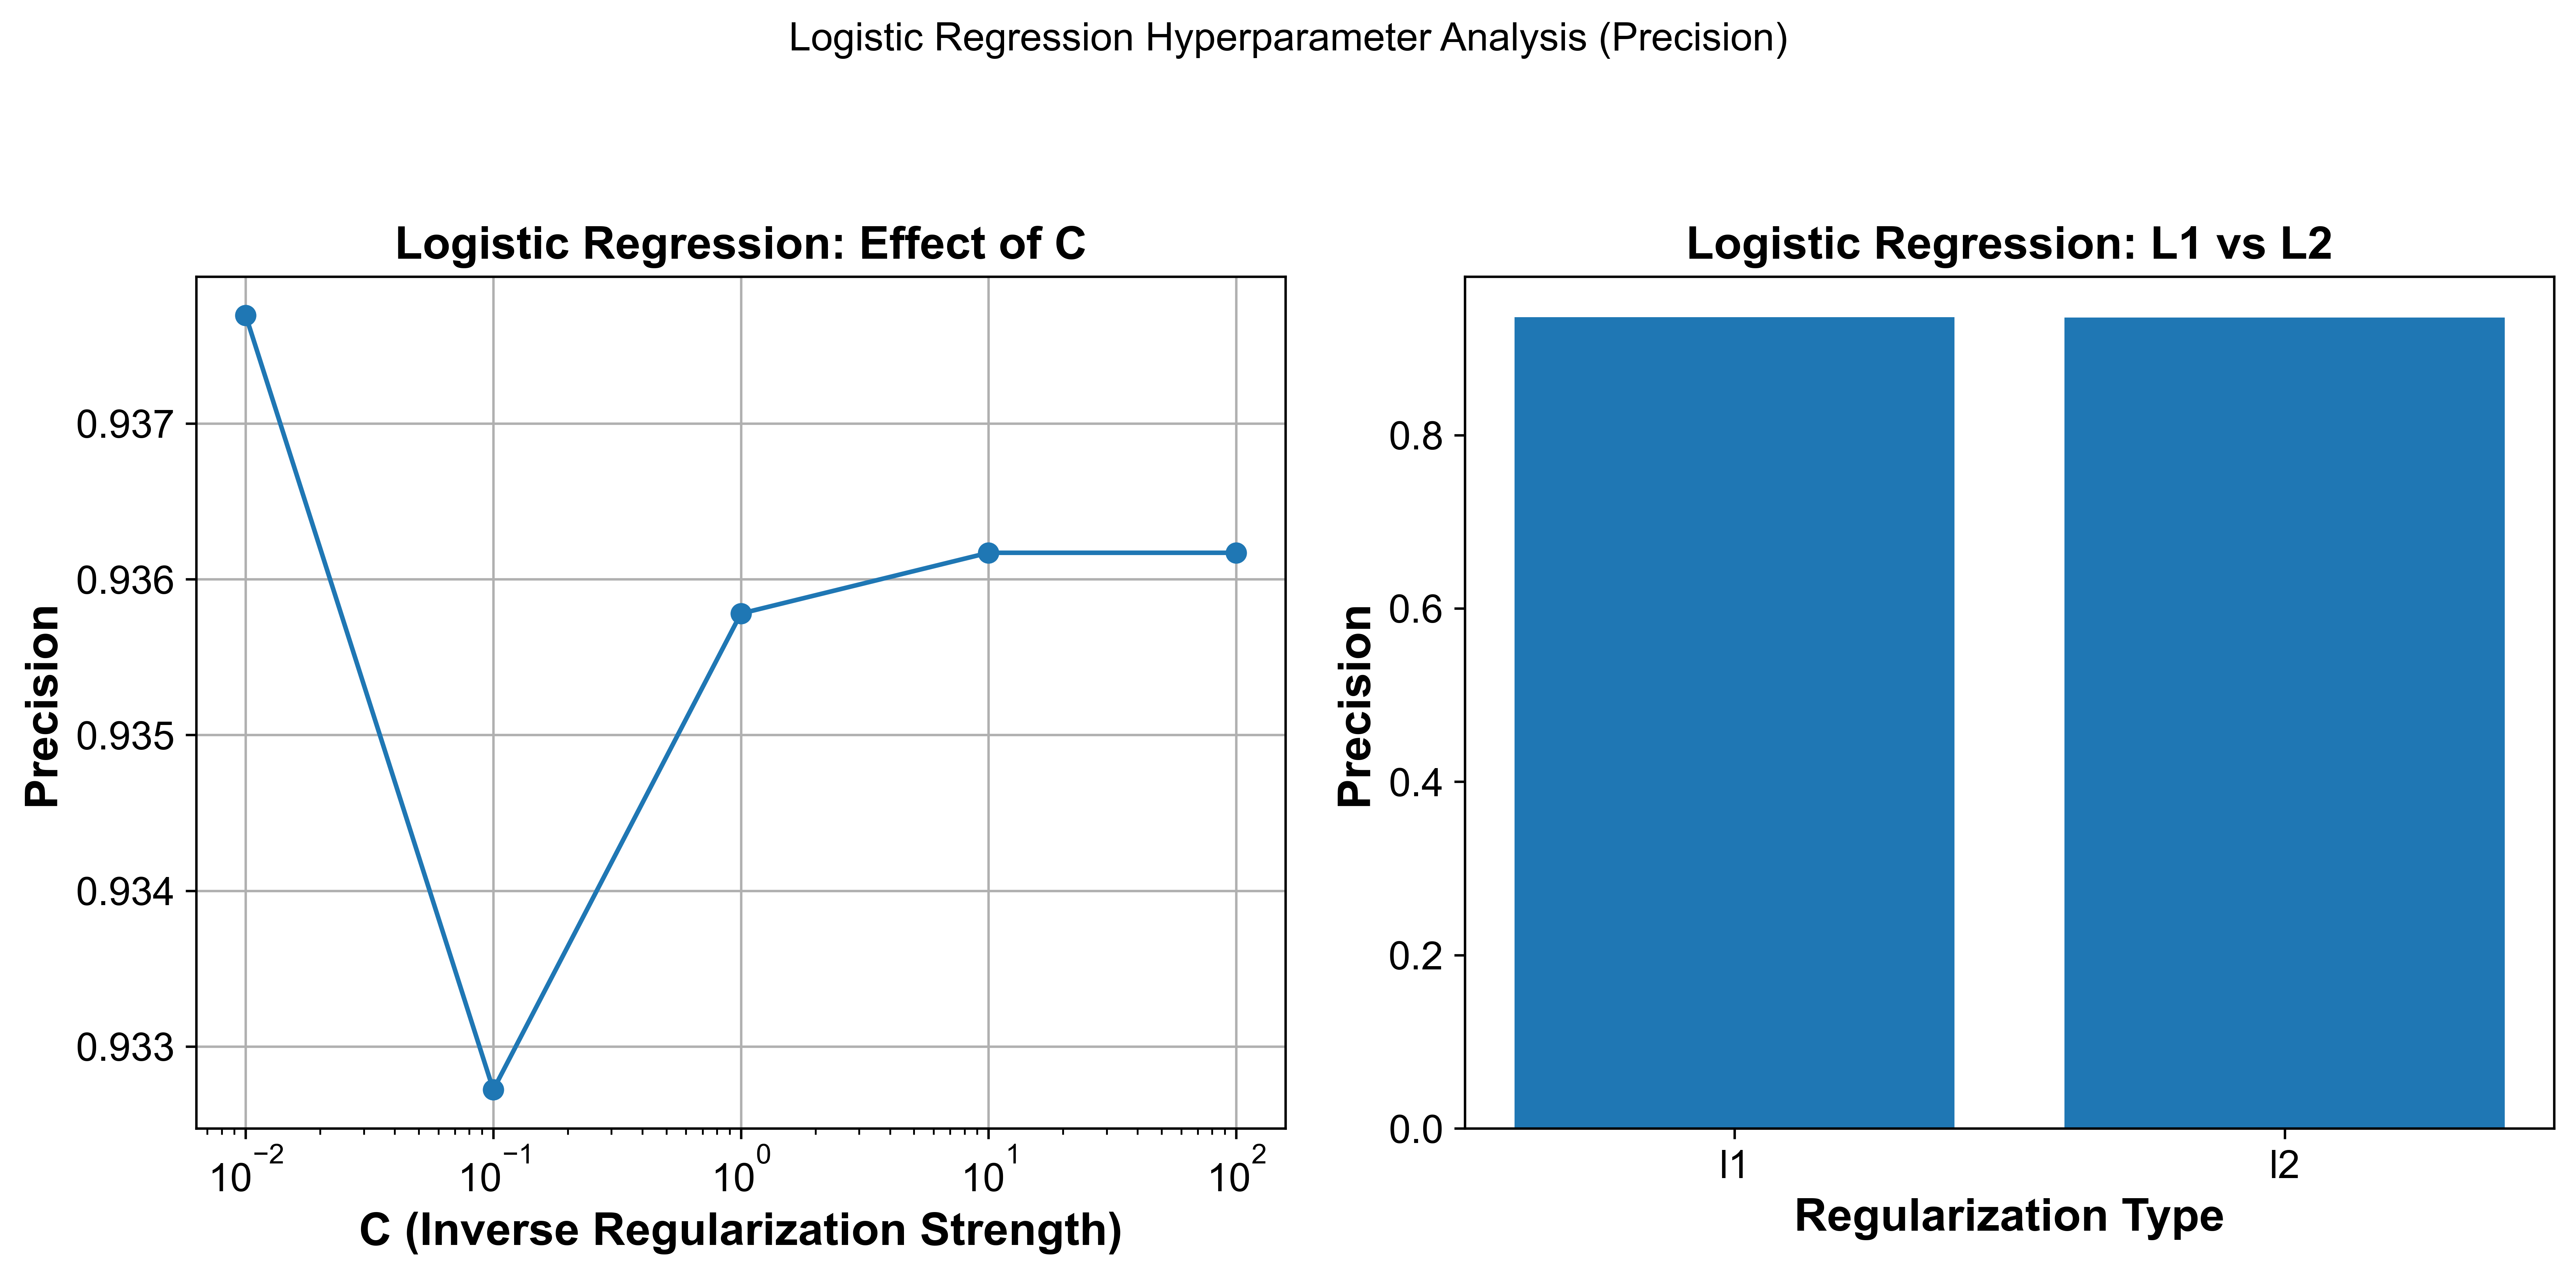
\includegraphics[width=\textwidth]{LR_hyperparameter_analysis.png}
    \caption{Logistic Regression HyperParameter Analysis}
\end{figure}

\begin{figure}[H]
    \centering
    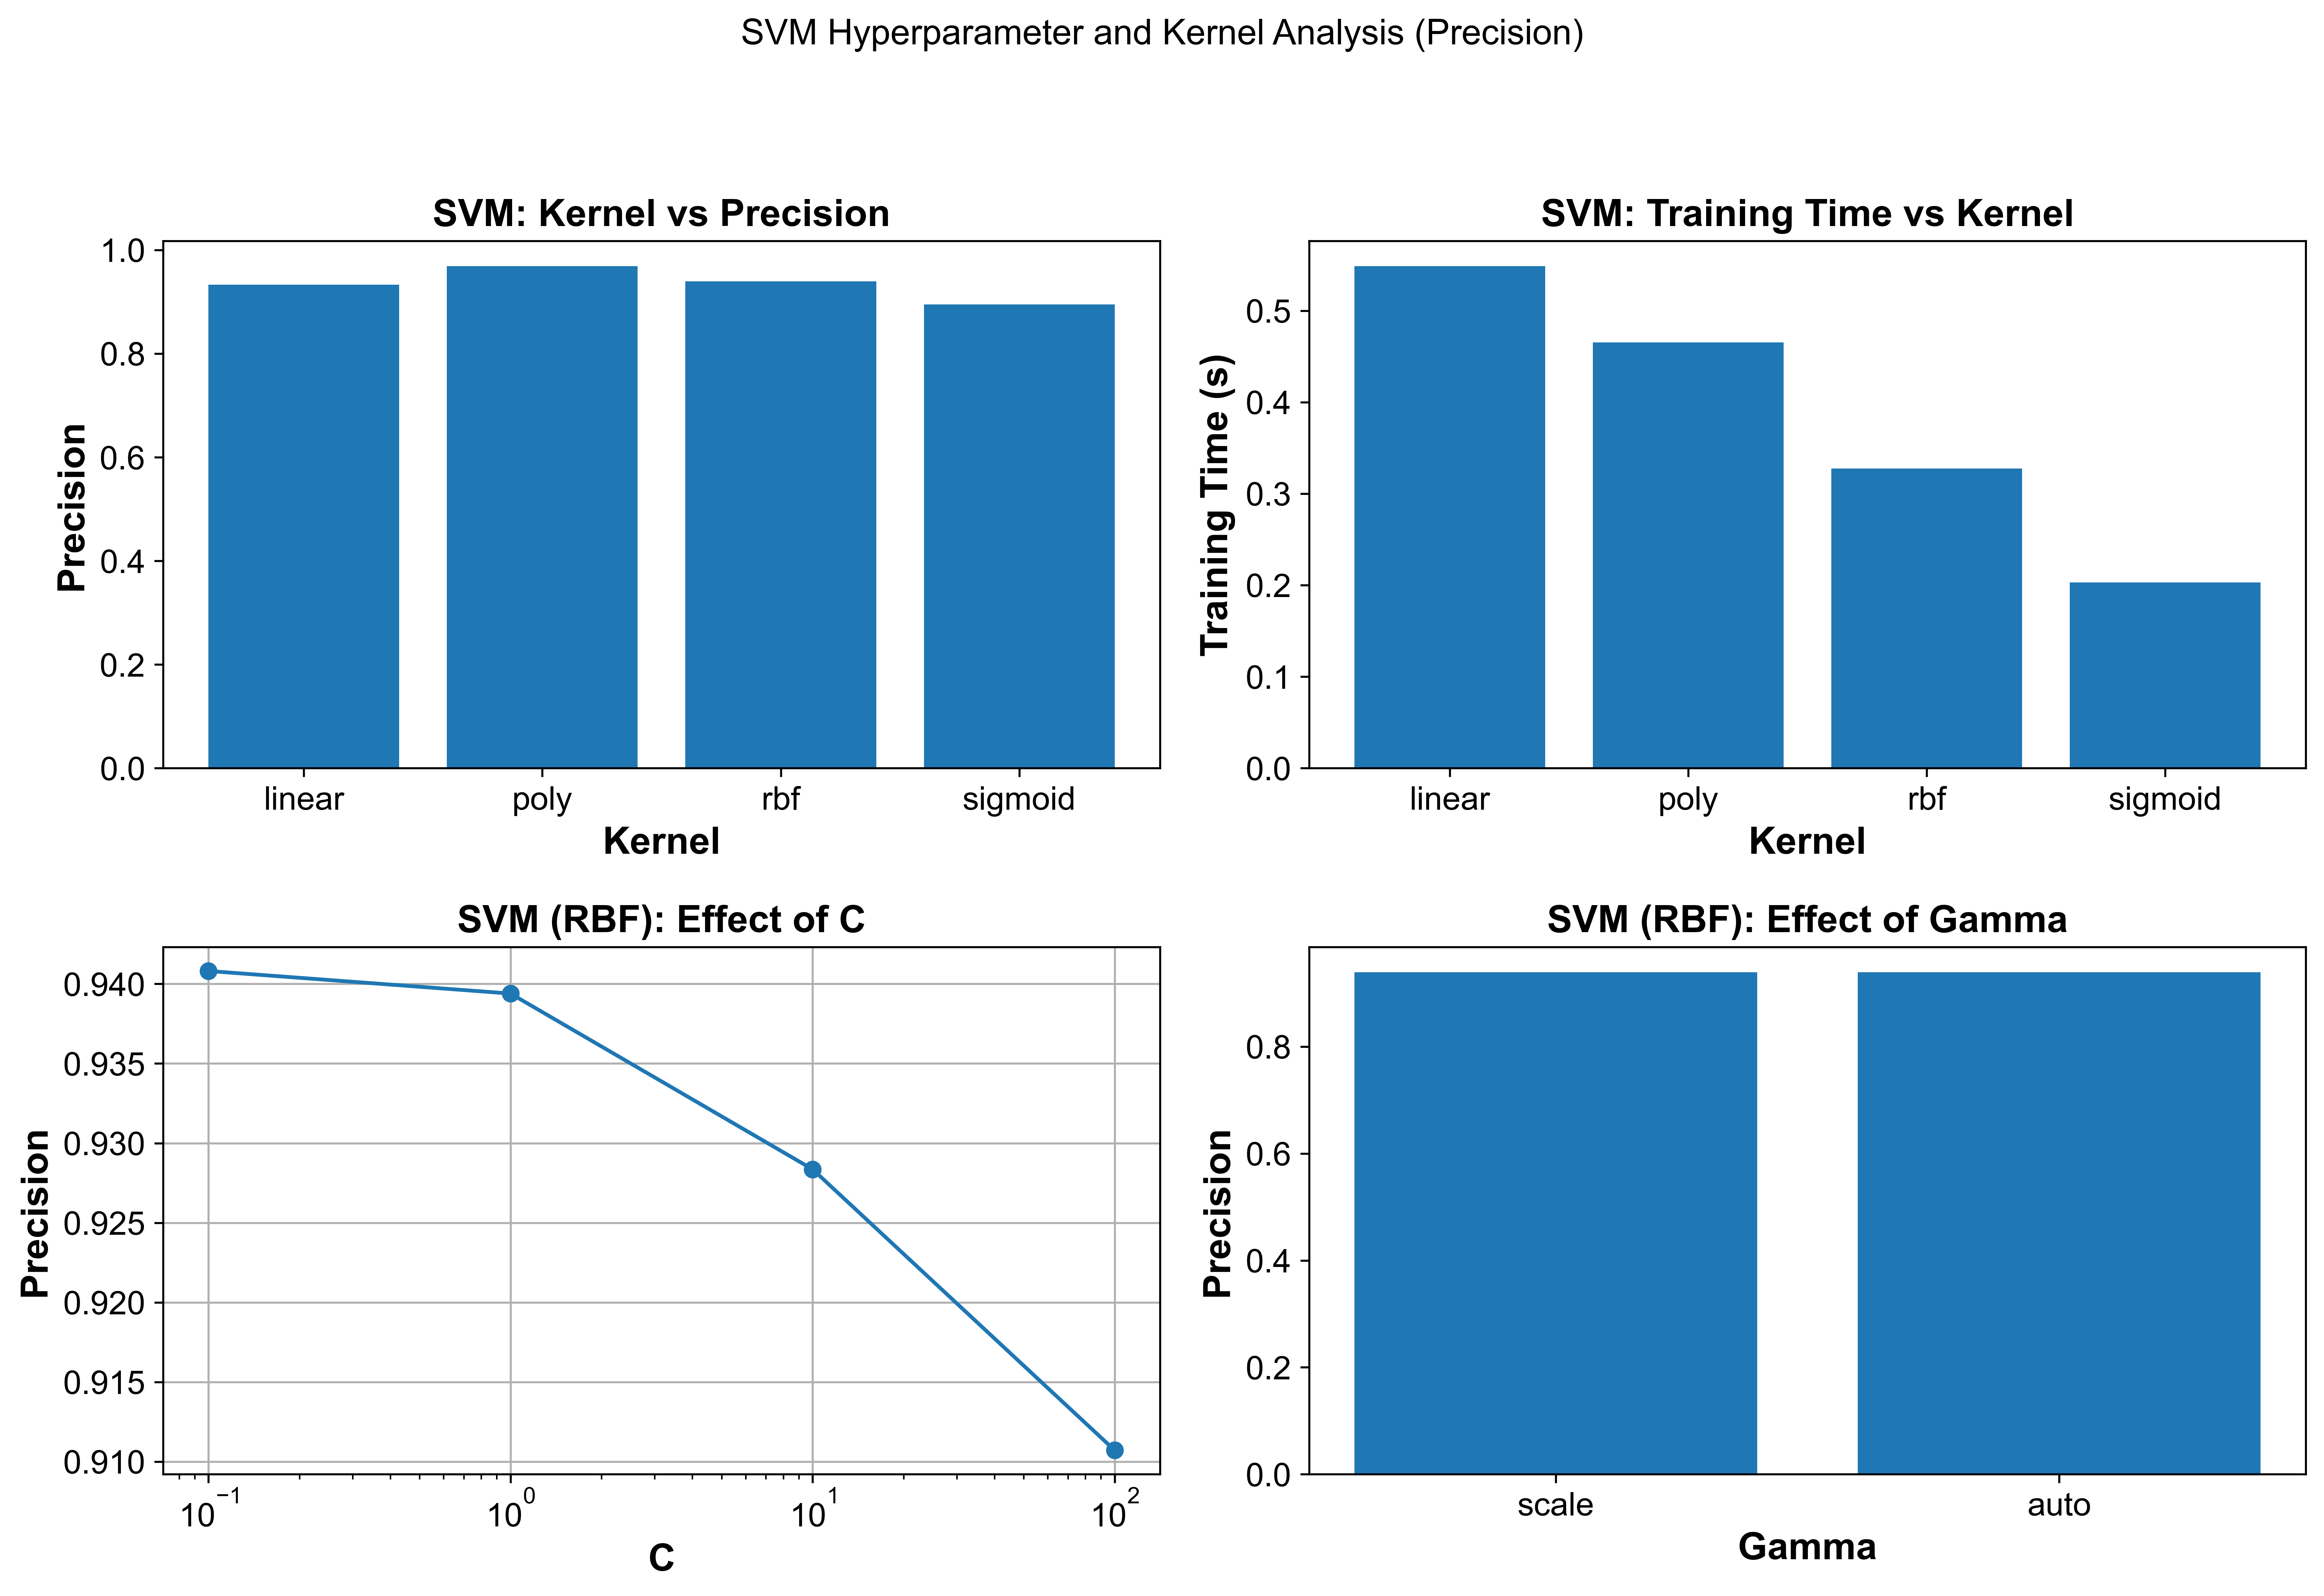
\includegraphics[width=\textwidth]{SVM_hyperparameter_analysis.png}
    \caption{Support Vector Machine HyperParameter Analysis}
\end{figure}


%==================================================
\section{Performance Tables}
%==================================================
%==================================================
\section*{Hyperparameter Tuning Results}
\begin{table}[H]
\centering
\renewcommand{\arraystretch}{1.3}
\begin{tabular}{|l|c|c|c|}
\hline
Model & Search Method & Best Parameters & Best CV Precision \\ \hline
Logistic Reg & Grid & 'C': 0.01, 'L1\_Ratio': 0.0 & 0.94 \\
Logistic Reg & Random & 'C': 0.002, 'L1\_Ratio': 0.0 & 0.95 \\
SVM & Grid & 'C': 0.1, 'degree': 4, 'gamma': 'auto', 'kernel': 'poly' & 0.99 \\
SVM & Random & 'C': 0.17, 'degree': 3, 'gamma': 'auto', 'kernel': 'poly' & 0.98 \\ \hline
\end{tabular}
\end{table}

%==================================================
\section*{Logistic Regression Performance}
\begin{table}[H]
\centering
\renewcommand{\arraystretch}{1.3}
\begin{tabular}{|l|c|}
\hline
Metric & Value \\ \hline
Accuracy & 0.92 \\
Precision & 0.96 \\
Recall & 0.85 \\
F1 Score & 0.90 \\
Training Time (s) & 0.02 \\ \hline
\end{tabular}
\end{table}

%==================================================
\section*{SVM Kernel-wise Performance}
\begin{table}[H]
\centering
\renewcommand{\arraystretch}{1.3}
\caption{Kernel-wise Performance Comparison of SVM}
\begin{tabular}{|l|c|c|c|c|}
\hline
\textbf{Kernel} & \textbf{Accuracy} & \textbf{Precision} & \textbf{F1 Score} & \textbf{Training Time (s)} \\ 
\hline
Linear & 0.94 & 0.93 & 0.92 & 0.35 \\
Polynomial & 0.92 & 0.97 & 0.90 & 0.19 \\
RBF & 0.94 & 0.94 & 0.93 & 0.20 \\
Sigmoid & 0.91 & 0.89 & 0.89 & 0.13 \\ 
\hline
\end{tabular}
\end{table}

%==================================================
\section*{K-Fold Cross-Validation Results (K = 5)}
\begin{table}[H]
\centering
\renewcommand{\arraystretch}{1.3}
\begin{tabular}{|c|c|c|}
\hline
Fold & Logistic Regression & SVM \\ \hline
Fold 1 & 0.95 & 0.99 \\
Fold 2 & 0.96 & 1.00 \\
Fold 3 & 0.95 & 1.00 \\
Fold 4 & 0.94 & 1.00 \\
Fold 5 & 0.95 & 0.99 \\ \hline
Average & 0.95 & 0.99 \\ \hline
\end{tabular}
\end{table}

%==================================================
\section*{Comparative Analysis}
\begin{table}[H]
\centering
\renewcommand{\arraystretch}{1.3}
\begin{tabular}{|l|c|c|}
\hline
Criterion & Logistic Regression & SVM \\ \hline
Precision & 0.95 & 0.99 \\
Model Complexity & Low & High \\
Training Time & Low & High \\
Interpretability & High & Low \\ \hline
\end{tabular}
\end{table}

%==================================================
\section{Observations}
\begin{itemize}
    \item The SVM classifier with RBF kernel achieves the best overall performance,
    showing high precision and balanced F1-score on the imbalanced email dataset.

    \item Regularization significantly affects model performance by controlling
    complexity; optimal values of the parameter $C$ improve precision while preventing
    overfitting.

    \item Different SVM kernels exhibit varied behavior, with non-linear kernels
    capturing complex data patterns more effectively than linear kernels.

    \item Proper hyperparameter tuning helps achieve a balanced bias--variance
    trade-off, resulting in improved generalization on unseen email data.
\end{itemize}

\section{Learning Outcomes}
\begin{itemize}
    \item Understand probabilistic and margin-based classifiers.
    \item Apply hyperparameter tuning.
    \item Evaluate classification models.
    \item Interpret experimental results.
\end{itemize}

\end{document}